\section{Variabilidad muestral y Teorema Central del Límite}
Muchas veces no podemos (ni debemos) encuestar o examinar a toda la población: tomamos una
muestra (un grupo chico de alumnos) para intentar inferir cómo le fue al conjunto completo. Aquí
surge una pregunta clave: si elegimos varios grupos de alumnos al azar, ¿todos los grupos tendrán
el mismo promedio? La respuesta es no, y a ese fenómeno lo llamamos variabilidad muestral. En
esta sección simularemos este comportamiento sobre la variable \Variable{chemistry\_score}, que
corresponde al examen de química de los estudiantes.

\AnalisisDescriptivo
Para montar la simulación necesitamos los parámetros reales de la población:
\begin{TablaDatosFlexible}{L{0.24\linewidth} C{0.14\linewidth} L{0.54\linewidth}}{\textbf{Parámetro} & \textbf{Valor} & \textbf{Interpretación}}

\TablaFilaFlexible{Variable analizada & \TablaClave{chemistry\_score} & Puntaje obtenido en el examen de química de los estudiantes.}
\TablaFilaFlexible{Cantidad de datos ($n$) & 111 & La población completa está compuesta por los 111 estudiantes de la base de datos.}
\TablaFilaFlexible{Media ($\mu$) & 81,37 & Es la calificación promedio real en química de toda la población.}
\TablaFilaFlexible{Desviación estándar ($\sigma$) & 5,26 & Mide qué tan dispersas están las notas individuales de química respecto a su promedio.}

\end{TablaDatosFlexible}

\subsection{La simulación}
La idea es sencilla: elegimos grupos (muestras) de distinto tamaño, calculamos el promedio de
cada grupo y observamos cómo se comportan esos promedios. Repetimos el experimento muchas veces
para cada tamaño y comparamos los resultados. Para cuantificar cuánto deben dispersarse los
promedios alrededor de la media real, la estadística utiliza el error estándar de la media:
\begin{equation*}
  \sigma_{\bar{x}} = \frac{\sigma}{\sqrt{n}}
\end{equation*}
\PalabraClave{Cómo se toman los datos:} Al crecer el tamaño del grupo $n$, el denominador
aumenta y el error estándar se reduce: los promedios muestrales se ven obligados a apretarse
alrededor del valor real de la población.

\subsection{Grupos chicos ($n = 10$)}
Seleccionamos 10 grupos de 10 alumnos cada uno y registramos sus promedios:

\TablaDeDatos
\begin{TablaDatosFlexible}
  {
    C{0.09\linewidth}
    L{0.72\linewidth}
    C{0.10\linewidth}}
    {
      \textbf{Muestra} &
      \textbf{Notas seleccionadas (tamaño \(n = 10\))} &
      \textbf{Promedio}
    }

\TablaFilaFlexible{1 & 86, 78, 82, 78, 82, 86, 78, 75, 80, 82 & 80,70}
\TablaFilaFlexible{2 & 86, 78, 86, 80, 75, 85, 75, 75, 82, 86 & 80,80}
\TablaFilaFlexible{3 & 87, 86, 87, 80, 78, 85, 90, 75, 90, 75 & 83,30}
\TablaFilaFlexible{4 & 80, 80, 75, 82, 85, 75, 86, 80, 86, 75 & 80,40}
\TablaFilaFlexible{5 & 75, 78, 78, 78, 78, 90, 78, 87, 90, 78 & 81,00}
\TablaFilaFlexible{6 & 80, 87, 78, 82, 90, 86, 75, 80, 87, 78 & 82,30}
\TablaFilaFlexible{7 & 88, 78, 80, 75, 80, 80, 78, 80, 82, 86 & 80,70}
\TablaFilaFlexible{8 & 78, 78, 90, 82, 87, 78, 80, 90, 78, 80 & 82,10}
\TablaFilaFlexible{9 & 78, 90, 78, 80, 78, 80, 82, 86, 78, 75 & 80,50}
\TablaFilaFlexible{10 & 78, 78, 80, 90, 86, 78, 87, 87, 75, 82 & 82,10}

\end{TablaDatosFlexible}


\PalabraClave{Lectura de la tabla:} Como son grupos chicos, los promedios están dispersos en un
rango de 80,40 a 83,30. Al haber pocos alumnos, cualquier nota extrema pesa demasiado en el
promedio y lo hace saltar. Aun así, el promedio global de estas 10 muestras da 81,39, rondando
la media real (81,37).

% --------------------------------------------------------------------------------------------------

\subsection{Grupos medianos ($n = 20$)}
Ampliamos el experimento a 20 grupos de 20 alumnos cada uno:

\TablaDeDatos
\begin{TablaDatosFlexible}
  {
    C{0.09\linewidth}
    L{0.72\linewidth}
    C{0.10\linewidth}}
    {
      \textbf{Muestra} &
      \textbf{Notas seleccionadas (tamaño \(n = 20\))} &
      \textbf{Promedio}
    }

\TablaFilaFlexible{1 & 78, 85, 87, 78, 78, 88, 78, 86, 75, 82, 78, 87, 78, 90, 90, 78, 90, 80, 90, 86 & 83,10}
\TablaFilaFlexible{2 & 80, 78, 87, 80, 90, 86, 75, 80, 78, 90, 75, 78, 82, 87, 75, 80, 82, 90, 78, 90 & 82,05}
\TablaFilaFlexible{3 & 90, 80, 78, 86, 75, 87, 75, 80, 80, 78, 78, 80, 78, 80, 78, 75, 80, 78, 86, 85 & 80,35}
\TablaFilaFlexible{4 & 78, 78, 78, 78, 75, 90, 78, 75, 80, 80, 82, 75, 78, 75, 75, 86, 78, 80, 86, 90 & 79,75}
\TablaFilaFlexible{5 & 78, 90, 82, 90, 90, 75, 87, 90, 85, 80, 90, 90, 80, 78, 78, 75, 90, 90, 78, 78 & 83,70}
\TablaFilaFlexible{6 & 78, 80, 87, 78, 78, 86, 90, 75, 82, 90, 75, 75, 78, 75, 78, 82, 78, 87, 90, 90 & 81,60}
\TablaFilaFlexible{7 & 82, 78, 88, 75, 82, 80, 78, 80, 78, 80, 90, 75, 87, 80, 78, 90, 78, 75, 82, 75 & 80,55}
\TablaFilaFlexible{8 & 86, 90, 78, 90, 80, 90, 78, 90, 80, 80, 80, 86, 86, 75, 75, 86, 80, 75, 78, 78 & 82,05}
\TablaFilaFlexible{9 & 80, 90, 90, 78, 90, 85, 90, 90, 88, 75, 87, 78, 86, 75, 82, 90, 75, 90, 80, 78 & 83,85}
\TablaFilaFlexible{10 & 80, 78, 90, 78, 86, 90, 78, 90, 90, 78, 78, 90, 78, 75, 80, 80, 90, 85, 75, 80 & 82,45}
\TablaFilaFlexible{11 & 75, 75, 80, 86, 78, 78, 75, 86, 86, 80, 80, 78, 78, 90, 75, 75, 87, 82, 82, 78 & 80,20}
\TablaFilaFlexible{12 & 87, 78, 80, 78, 80, 80, 75, 86, 75, 78, 87, 82, 90, 80, 90, 80, 90, 78, 78, 90 & 82,10}
\TablaFilaFlexible{13 & 80, 78, 90, 75, 87, 87, 80, 90, 80, 78, 80, 87, 86, 78, 82, 90, 78, 78, 90, 85 & 82,95}
\TablaFilaFlexible{14 & 78, 90, 78, 78, 75, 78, 78, 78, 86, 86, 80, 78, 87, 80, 78, 78, 86, 75, 90, 90 & 81,35}
\TablaFilaFlexible{15 & 90, 90, 90, 78, 80, 75, 80, 86, 80, 80, 80, 80, 78, 78, 90, 87, 75, 87, 78, 86 & 82,40}
\TablaFilaFlexible{16 & 78, 75, 78, 78, 82, 75, 75, 75, 78, 86, 75, 78, 87, 78, 90, 75, 82, 87, 78, 78 & 79,40}
\TablaFilaFlexible{17 & 90, 78, 87, 80, 78, 80, 90, 75, 78, 75, 78, 90, 80, 78, 80, 80, 75, 90, 75, 78 & 80,75}
\TablaFilaFlexible{18 & 75, 78, 78, 80, 75, 85, 90, 75, 80, 87, 80, 86, 75, 87, 78, 78, 78, 75, 80, 80 & 80,00}
\TablaFilaFlexible{19 & 87, 75, 80, 82, 80, 82, 86, 78, 86, 78, 80, 80, 75, 80, 90, 78, 78, 90, 86, 78 & 81,45}
\TablaFilaFlexible{20 & 82, 80, 86, 75, 80, 86, 80, 90, 78, 78, 78, 78, 86, 80, 75, 78, 75, 78, 90, 90 & 81,15}

\end{TablaDatosFlexible}


\PalabraClave{Lectura de la tabla:} Al agrandar el grupo, las notas altas y bajas empiezan a
compensarse entre sí. Aunque el azar puede hacer que alguna tanda salga más movida (en esta
simulación los promedios oscilaron entre 79,40 y 83,85), el promedio de medias da 81,56,
manteniéndose muy cerca del parámetro real.

% --------------------------------------------------------------------------------------------------

\subsection{Grupos óptimos ($n = 30$)}
Por último, simulamos 30 grupos de 30 alumnos cada uno, alcanzando el mínimo que establece la
regla estadística para aplicar el Teorema Central del Límite:

\TablaDeDatos
\begin{TablaDatosFlexible}
  {
    C{0.09\linewidth}
    L{0.72\linewidth}
    C{0.10\linewidth}}
    {
      \textbf{Muestra} &
      \textbf{Notas seleccionadas (tamaño \(n = 30\))} &
      \textbf{Promedio}
    }

\TablaFilaFlexible{1 & 87, 78, 87, 80, 90, 75, 78, 78, 87, 80, 82, 78, 78, 80, 78, 78, 75, 90, 86, 78, 80, 78, 90, 90, 78, 80, 78, 82, 85, 75 & 81,30}
\TablaFilaFlexible{2 & 75, 90, 75, 78, 80, 85, 75, 86, 75, 78, 78, 80, 80, 87, 75, 86, 86, 78, 78, 90, 80, 78, 78, 75, 75, 78, 86, 90, 90, 75 & 80,67}
\TablaFilaFlexible{3 & 75, 75, 75, 78, 78, 90, 75, 87, 78, 78, 87, 80, 75, 75, 75, 86, 87, 75, 85, 90, 78, 86, 78, 75, 80, 75, 80, 86, 80, 85 & 80,23}
\TablaFilaFlexible{4 & 82, 78, 78, 78, 78, 80, 78, 90, 75, 90, 78, 78, 75, 90, 78, 82, 82, 87, 75, 86, 80, 90, 86, 90, 78, 90, 80, 75, 80, 86 & 81,77}
\TablaFilaFlexible{5 & 86, 90, 80, 80, 86, 86, 78, 75, 75, 82, 82, 75, 80, 85, 90, 75, 75, 80, 75, 78, 78, 78, 90, 80, 90, 90, 80, 87, 75, 75 & 81,20}
\TablaFilaFlexible{6 & 78, 78, 80, 80, 90, 87, 90, 80, 75, 86, 86, 78, 86, 80, 82, 90, 75, 90, 78, 78, 90, 82, 90, 86, 80, 78, 75, 78, 80, 78 & 82,13}
\TablaFilaFlexible{7 & 75, 78, 78, 90, 75, 82, 78, 90, 90, 82, 75, 78, 78, 75, 80, 78, 86, 85, 80, 75, 78, 87, 80, 90, 90, 75, 90, 86, 90, 80 & 81,80}
\TablaFilaFlexible{8 & 75, 78, 80, 80, 78, 75, 86, 78, 78, 80, 75, 78, 75, 78, 75, 78, 78, 86, 86, 80, 90, 90, 78, 80, 78, 78, 75, 90, 75, 78 & 79,63}
\TablaFilaFlexible{9 & 86, 75, 90, 78, 78, 82, 78, 80, 80, 86, 78, 78, 78, 86, 80, 78, 78, 75, 75, 87, 75, 87, 90, 80, 80, 82, 75, 78, 80, 88 & 80,70}
\TablaFilaFlexible{10 & 90, 90, 75, 75, 78, 78, 78, 80, 78, 78, 78, 78, 75, 78, 90, 80, 86, 87, 85, 82, 78, 75, 75, 90, 80, 75, 75, 75, 80, 86 & 80,27}
\TablaFilaFlexible{11 & 87, 75, 78, 82, 75, 75, 78, 90, 78, 90, 86, 78, 78, 86, 78, 90, 75, 78, 86, 85, 78, 90, 87, 86, 78, 78, 82, 75, 80, 80 & 81,40}
\TablaFilaFlexible{12 & 75, 78, 80, 86, 82, 86, 78, 75, 78, 90, 78, 78, 87, 90, 87, 75, 75, 75, 80, 90, 75, 80, 80, 78, 80, 86, 80, 90, 87, 86 & 81,50}
\TablaFilaFlexible{13 & 78, 87, 80, 78, 90, 78, 78, 78, 87, 86, 88, 75, 75, 82, 90, 78, 78, 80, 75, 78, 82, 87, 80, 75, 80, 78, 86, 80, 75, 75 & 80,57}
\TablaFilaFlexible{14 & 80, 87, 86, 86, 90, 75, 80, 75, 78, 78, 75, 82, 78, 80, 90, 90, 78, 78, 75, 78, 90, 90, 90, 78, 78, 80, 80, 75, 78, 80 & 81,27}
\TablaFilaFlexible{15 & 75, 80, 78, 75, 75, 86, 75, 80, 90, 78, 90, 75, 75, 86, 80, 87, 90, 90, 78, 78, 75, 75, 80, 78, 82, 90, 86, 78, 78, 78 & 80,70}
\TablaFilaFlexible{16 & 80, 90, 80, 75, 78, 80, 80, 75, 78, 78, 80, 86, 82, 82, 78, 90, 87, 78, 80, 75, 78, 80, 75, 78, 75, 78, 75, 82, 80, 85 & 79,93}
\TablaFilaFlexible{17 & 90, 82, 87, 80, 78, 75, 80, 80, 75, 90, 86, 90, 78, 90, 90, 78, 86, 78, 82, 85, 75, 78, 75, 75, 87, 87, 87, 82, 90, 86 & 82,73}
\TablaFilaFlexible{18 & 78, 75, 78, 80, 75, 86, 87, 78, 86, 78, 80, 85, 82, 80, 80, 80, 78, 78, 80, 75, 86, 90, 78, 75, 87, 78, 78, 75, 86, 86 & 80,60}
\TablaFilaFlexible{19 & 90, 80, 78, 78, 80, 86, 75, 78, 80, 78, 87, 90, 82, 86, 78, 80, 78, 87, 86, 86, 78, 75, 87, 87, 78, 90, 90, 75, 80, 78 & 82,03}
\TablaFilaFlexible{20 & 80, 82, 78, 78, 75, 78, 82, 80, 90, 75, 78, 88, 90, 90, 86, 78, 78, 78, 90, 86, 75, 78, 80, 75, 85, 90, 80, 80, 80, 90 & 81,77}
\TablaFilaFlexible{21 & 78, 90, 75, 86, 80, 90, 80, 87, 75, 80, 75, 90, 90, 78, 82, 80, 78, 87, 78, 78, 78, 80, 90, 75, 78, 80, 75, 87, 80, 78 & 81,27}
\TablaFilaFlexible{22 & 90, 86, 75, 78, 75, 75, 80, 86, 75, 75, 87, 90, 82, 90, 90, 75, 78, 80, 78, 78, 87, 78, 80, 78, 78, 78, 82, 90, 78, 78 & 81,00}
\TablaFilaFlexible{23 & 75, 87, 78, 80, 82, 87, 86, 75, 90, 80, 78, 78, 75, 78, 90, 78, 87, 86, 90, 78, 80, 87, 90, 78, 75, 75, 80, 78, 90, 82 & 81,77}
\TablaFilaFlexible{24 & 78, 87, 75, 78, 86, 82, 90, 80, 78, 78, 78, 78, 87, 90, 78, 82, 90, 87, 90, 87, 78, 75, 80, 86, 75, 75, 90, 86, 78, 90 & 82,40}
\TablaFilaFlexible{25 & 80, 78, 82, 78, 75, 90, 87, 86, 90, 78, 90, 80, 78, 78, 90, 75, 78, 82, 75, 78, 90, 80, 75, 75, 75, 80, 90, 75, 78, 75 & 80,70}
\TablaFilaFlexible{26 & 86, 75, 75, 78, 78, 86, 80, 90, 80, 82, 75, 75, 80, 78, 90, 75, 80, 86, 78, 80, 90, 78, 75, 75, 82, 86, 82, 87, 85, 78 & 80,83}
\TablaFilaFlexible{27 & 78, 80, 80, 90, 86, 80, 78, 78, 75, 80, 78, 90, 86, 78, 90, 86, 87, 88, 78, 86, 87, 78, 75, 90, 87, 80, 86, 82, 87, 86 & 83,00}
\TablaFilaFlexible{28 & 78, 75, 87, 75, 80, 80, 87, 88, 78, 80, 75, 90, 90, 90, 75, 80, 75, 78, 78, 78, 75, 85, 75, 90, 80, 86, 78, 86, 75, 78 & 80,83}
\TablaFilaFlexible{29 & 80, 90, 75, 75, 80, 75, 78, 88, 80, 87, 86, 78, 78, 80, 90, 82, 86, 90, 86, 78, 87, 82, 78, 78, 75, 80, 85, 80, 78, 75 & 81,33}
\TablaFilaFlexible{30 & 86, 75, 87, 90, 85, 78, 90, 75, 90, 78, 80, 75, 80, 87, 80, 90, 78, 78, 75, 75, 90, 90, 75, 78, 87, 75, 82, 90, 75, 80 & 81,80}

\end{TablaDatosFlexible}


\PalabraClave{Lectura de la tabla:} Al alcanzar el tamaño óptimo, el error estándar cae
notablemente: el desvío de los promedios se reduce a 0,80 puntos, el más bajo de toda la
simulación. El promedio global de las 30 muestras es 81,24, demostrando la convergencia que
dicta el Teorema Central del Límite.

\subsection{Cuadro resumen}
Comparar los tres tamaños de grupo lado a lado permite ver el patrón completo de la simulación:

\begin{TablaDatosFlexible}{C{0.10\linewidth} C{0.12\linewidth} L{0.20\linewidth} C{0.15\linewidth} C{0.15\linewidth} C{0.14\linewidth}}{\textbf{Tamaño ($n$)} & \textbf{Muestras} & \textbf{Rango de promedios} & \textbf{Desvío de los promedios} & \textbf{Error estándar ($\frac{\sigma}{\sqrt{n}}$)} & \textbf{Promedio global}}

\TablaFilaFlexible{10 & 10 & 80,40 – 83,30 & 0,98 & 1,66 & 81,39}
\TablaFilaFlexible{20 & 20 & 79,40 – 83,85 & 1,30 & 1,18 & 81,56}
\TablaFilaFlexible{30 & 30 & 79,63 – 83,00 & 0,80 & 0,96 & 81,24}

\end{TablaDatosFlexible}

El desvío de los promedios observado en la simulación acompaña la tendencia que predice la
teoría: a medida que crece el tamaño del grupo $n$, el error estándar teórico
$\sigma / \sqrt{n}$ se reduce y los promedios se compactan alrededor de la media real
$\mu = 81{,}37$. Los tres promedios globales (81,39; 81,56 y 81,24) caen todos a menos de
0,20 puntos de la realidad, confirmando que la media muestral no sesga la estimación.

% --------------------------------------------------------------------------------------------------

\TituloGrafico{Distribución de los promedios muestrales}
Podemos visualizar el fenómeno dibujando la distribución teórica de los promedios para cada
tamaño de grupo. Como la varianza de los promedios es $\sigma^2 / n$, cada campana se dibuja
con centro en la media real y con un error estándar igual a $\sigma / \sqrt{n}$:

\begin{figure}[H]
    \centering
    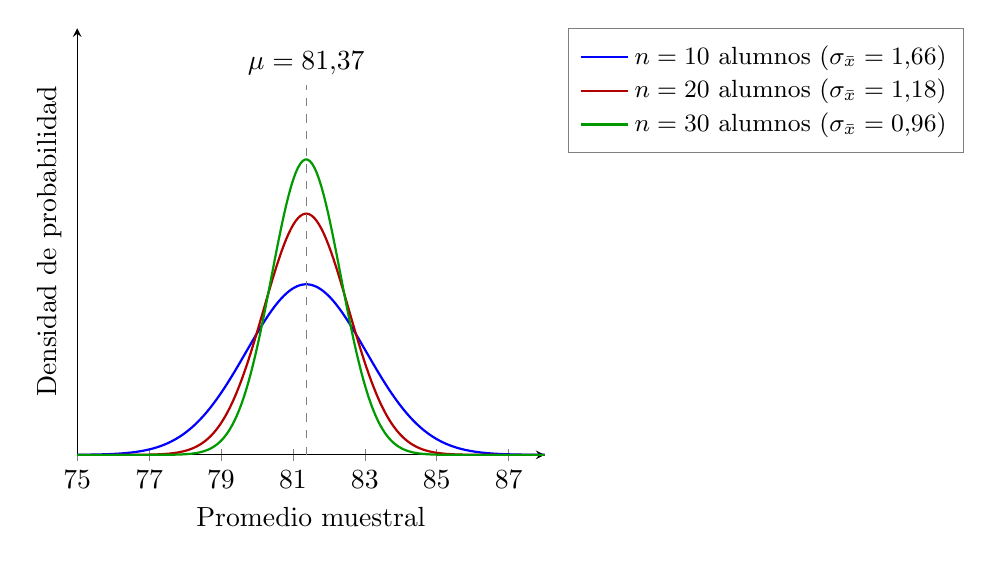
\begin{tikzpicture}
        % Función de densidad normal con parámetros configurables.
        \pgfmathdeclarefunction{dens}{3}{%
          \pgfmathparse{1/(#3*sqrt(2*pi))*exp(-((#1-#2)^2)/(2*(#3)^2))}%
        }
        \begin{axis}[
            width=0.62\textwidth,
            height=7cm,
            xlabel={Promedio muestral},
            ylabel={Densidad de probabilidad},
            xmin=75, xmax=88,
            ymin=0, ymax=0.6,
            xtick={75,77,79,81,83,85,87},
            ytick=\empty,
            axis lines=left,
            samples=200,
            legend style={at={(1.05,1.0)}, anchor=north west, font=\small,
                fill=white, draw=black!50, fill opacity=1, text opacity=1,
                inner sep=4pt, cells={anchor=west}},
            legend cell align=left,
            clip=false,
        ]
            % Campana para n = 10 (error estándar 1,66).
            \addplot[blue, thick, domain=75:88] {dens(x,81.37,1.6634)};
            \addlegendentry{$n = 10$ alumnos ($\sigma_{\bar{x}} = 1{,}66$)}
            % Campana para n = 20 (error estándar 1,18).
            \addplot[red!70!black, thick, domain=75:88] {dens(x,81.37,1.1762)};
            \addlegendentry{$n = 20$ alumnos ($\sigma_{\bar{x}} = 1{,}18$)}
            % Campana para n = 30 (error estándar 0,96).
            \addplot[green!60!black, thick, domain=75:88] {dens(x,81.37,0.9603)};
            \addlegendentry{$n = 30$ alumnos ($\sigma_{\bar{x}} = 0{,}96$)}
            % Media real de la población.
            \draw[dashed, gray] (axis cs:81.37,0) -- (axis cs:81.37,0.52)
                node[above, black] {$\mu = 81{,}37$};
        \end{axis}
    \end{tikzpicture}
    \caption{Distribución teórica de los promedios muestrales para los tres tamaños de grupo. A
    mayor tamaño $n$, la campana se vuelve más alta y delgada, concentrándose en la media real.}
    \label{fig:variabilidad_campanas}
\end{figure}

\PalabraClave{Análisis de las campanas:}
\begin{itemize}
  \item \textbf{La campana de $n = 10$ (azul):} Es la más ancha y baja. Sus promedios pueden
    alejarse de la media real hasta 1,66 puntos en promedio, reflejando la inestabilidad de los
    grupos chicos.
  \item \textbf{La campana de $n = 30$ (verde):} Es la más alta y delgada. Toda su masa se
    concentra en una franja estrecha alrededor de 81,37, lo que significa que casi cualquier
    muestra de ese tamaño dará un promedio muy cercano a la realidad.
  \item \textbf{Todas comparten el centro:} Las tres campanas están ancladas en la misma media
    $\mu = 81{,}37$. Ningún tamaño de grupo cambia el promedio esperado; solo cambia la
    precisión con la que se alcanza.
\end{itemize}

\subsection{¿Qué nos demuestra el Teorema Central del Límite?}
\PalabraClave{El promedio de los promedios no miente:} Si tomamos muchas muestras, la media de
todas ellas siempre va a converger hacia la media real de toda la población. En nuestra
simulación, los tres promedios globales dieron 81,39; 81,56 y 81,24, todos dentro de 0,20
puntos de los 81,37 reales.

\PalabraClave{A mayor grupo, mayor precisión:} Cuanto más grande sea la muestra que elijamos,
menor será la dispersión (el error estándar). Como muestra la fórmula
$\sigma_{\bar{x}} = \sigma / \sqrt{n}$, al pasar de 10 a 30 alumnos el error cae de 1,66 a
0,96 puntos: la campana se vuelve más alta y delgada, concentrándose en el valor real.

\PalabraClave{La forma siempre tiende a la normalidad:} No importa si las notas originales de
la escuela están amontonadas de forma extraña o asimétrica; los promedios de los grupos grandes
siempre se van a ordenar dibujando una campana de Gauss perfecta y simétrica.

\Interpretacion
Este tema nos demuestra que la media muestral $\bar{x}$ es el mejor estimador posible para
conocer la realidad de los alumnos: no solo no genera sesgo (sus promedios rondan siempre el
valor real), sino que, a mayor tamaño del grupo, su error de estimación se reduce de forma
controlada y predecible. En la práctica, esto justifica que la institución pueda
evaluar el nivel de química de toda la escuela confiando en grupos de 30 estudiantes, sin
necesidad de examinar a los 111 alumnos.


